%%%%%%%%%%%%%%%%%%%%%%%%%%%%%%%%%%%%%%%%%
% Article EcoFoG
% Version 2.1 (23/10/2017)
%
% adapté de :
% Stylish Article
% LaTeX Template
% Version 1.0 (31/1/13)
%
% This template has been downloaded from:
% http://www.LaTeXTemplates.com
%
% Original author:
% Mathias Legrand (legrand.mathias@gmail.com)
%
% License:
% CC BY-NC-SA 3.0 (http://creativecommons.org/licenses/by-nc-sa/3.0/)
%
%%%%%%%%%%%%%%%%%%%%%%%%%%%%%%%%%%%%%%%%%


%----------------------------------------------------------------------------------------
%	PACKAGES AND OTHER DOCUMENT CONFIGURATIONS
%----------------------------------------------------------------------------------------

\documentclass[fleqn,10pt]{ArtEcoFoG} % Document font size and equations flushed left

\setcounter{tocdepth}{3} % Show only three levels in the table of contents section: sections, subsections and subsubsections


% Pandoc environments
\usepackage{framed}
\usepackage{fancyvrb}
\providecommand{\tightlist}{%
  \setlength{\itemsep}{0pt}\setlength{\parskip}{0pt}}
\newcommand{\VerbBar}{|}
\newcommand{\VERB}{\Verb[commandchars=\\\{\}]}
\DefineVerbatimEnvironment{Highlighting}{Verbatim}{commandchars=\\\{\}, fontsize=\scriptsize} % Code R
\definecolor{shadecolor}{RGB}{248,248,248}
\newenvironment{Shaded}{\begin{snugshade}}{\end{snugshade}}
\newcommand{\KeywordTok}[1]{\textcolor[rgb]{0.13,0.29,0.53}{\textbf{{#1}}}}
\newcommand{\DataTypeTok}[1]{\textcolor[rgb]{0.13,0.29,0.53}{{#1}}}
\newcommand{\DecValTok}[1]{\textcolor[rgb]{0.00,0.00,0.81}{{#1}}}
\newcommand{\BaseNTok}[1]{\textcolor[rgb]{0.00,0.00,0.81}{{#1}}}
\newcommand{\FloatTok}[1]{\textcolor[rgb]{0.00,0.00,0.81}{{#1}}}
\newcommand{\ConstantTok}[1]{\textcolor[rgb]{0.00,0.00,0.00}{{#1}}}
\newcommand{\CharTok}[1]{\textcolor[rgb]{0.31,0.60,0.02}{{#1}}}
\newcommand{\SpecialCharTok}[1]{\textcolor[rgb]{0.00,0.00,0.00}{{#1}}}
\newcommand{\StringTok}[1]{\textcolor[rgb]{0.31,0.60,0.02}{{#1}}}
\newcommand{\VerbatimStringTok}[1]{\textcolor[rgb]{0.31,0.60,0.02}{{#1}}}
\newcommand{\SpecialStringTok}[1]{\textcolor[rgb]{0.31,0.60,0.02}{{#1}}}
\newcommand{\ImportTok}[1]{{#1}}
\newcommand{\CommentTok}[1]{\textcolor[rgb]{0.56,0.35,0.01}{\textit{{#1}}}}
\newcommand{\DocumentationTok}[1]{\textcolor[rgb]{0.56,0.35,0.01}{\textbf{\textit{{#1}}}}}
\newcommand{\AnnotationTok}[1]{\textcolor[rgb]{0.56,0.35,0.01}{\textbf{\textit{{#1}}}}}
\newcommand{\CommentVarTok}[1]{\textcolor[rgb]{0.56,0.35,0.01}{\textbf{\textit{{#1}}}}}
\newcommand{\OtherTok}[1]{\textcolor[rgb]{0.56,0.35,0.01}{{#1}}}
\newcommand{\FunctionTok}[1]{\textcolor[rgb]{0.00,0.00,0.00}{{#1}}}
\newcommand{\VariableTok}[1]{\textcolor[rgb]{0.00,0.00,0.00}{{#1}}}
\newcommand{\ControlFlowTok}[1]{\textcolor[rgb]{0.13,0.29,0.53}{\textbf{{#1}}}}
\newcommand{\OperatorTok}[1]{\textcolor[rgb]{0.81,0.36,0.00}{\textbf{{#1}}}}
\newcommand{\BuiltInTok}[1]{{#1}}
\newcommand{\ExtensionTok}[1]{{#1}}
\newcommand{\PreprocessorTok}[1]{\textcolor[rgb]{0.56,0.35,0.01}{\textit{{#1}}}}
\newcommand{\AttributeTok}[1]{\textcolor[rgb]{0.77,0.63,0.00}{{#1}}}
\newcommand{\RegionMarkerTok}[1]{{#1}}
\newcommand{\InformationTok}[1]{\textcolor[rgb]{0.56,0.35,0.01}{\textbf{\textit{{#1}}}}}
\newcommand{\WarningTok}[1]{\textcolor[rgb]{0.56,0.35,0.01}{\textbf{\textit{{#1}}}}}
\newcommand{\AlertTok}[1]{\textcolor[rgb]{0.94,0.16,0.16}{{#1}}}
\newcommand{\ErrorTok}[1]{\textcolor[rgb]{0.64,0.00,0.00}{\textbf{{#1}}}}
\newcommand{\NormalTok}[1]{{#1}}
\usepackage{longtable,booktabs}
\usepackage{caption}
% These lines are needed to make table captions work with longtable:
\makeatletter
\def\fnum@table{\tablename~\thetable}
\makeatother
% longtable 2 columns
% https://tex.stackexchange.com/questions/161431/how-to-solve-longtable-is-not-in-1-column-mode-error
\makeatletter
\let\oldlt\longtable
\let\endoldlt\endlongtable
\def\longtable{\@ifnextchar[\longtable@i \longtable@ii}
\def\longtable@i[#1]{\begin{figure}[t]
\onecolumn
\begin{minipage}{0.5\textwidth}\scriptsize
\oldlt[#1]
}
\def\longtable@ii{\begin{figure}[t]
\onecolumn
\begin{minipage}{0.5\textwidth}\scriptsize
\oldlt
}
\def\endlongtable{\endoldlt
\end{minipage}
\twocolumn
\end{figure}}
\makeatother

\usepackage{graphicx,grffile}
\makeatletter
\def\maxwidth{\ifdim\Gin@nat@width>\linewidth\linewidth\else\Gin@nat@width\fi}
\def\maxheight{\ifdim\Gin@nat@height>\textheight0.8\textheight\else\Gin@nat@height\fi}
\makeatother
% Scale images if necessary, so that they will not overflow the page
% margins by default, and it is still possible to overwrite the defaults
% using explicit options in \includegraphics[width, height, ...]{}
\setkeys{Gin}{width=\maxwidth,height=\maxheight,keepaspectratio}

% User-adder preamble
\usepackage{textcomp} \DeclareUnicodeCharacter{B0}{\textdegree}
\hyphenation{sa-plings} \usepackage{longtable,tabu}

%----------------------------------------------------------------------------------------
%	ARTICLE INFORMATION
%----------------------------------------------------------------------------------------

\JournalInfo{Hal xxxx} % Journal information
\Archive{DOI xxxx} % Additional notes (e.g. copyright, DOI, review/research article)

\PaperTitle{Inescapable Taxonomists: Workable Biodiversity Management Must Base on a
Minimum Field Work} % Article title

\Authors{
Ariane Mirabel\textsuperscript{1*}\\ Eric Marcon\textsuperscript{1}\\ Bruno Hérault\textsuperscript{2}
} % Authors
\affiliation{
\textsuperscript{1}UMR EcoFoG, AgroParistech, CNRS, Cirad, INRA, Université des Antilles,
Université de Guyane.\\ \hspace{1em} Campus Agronomique, 97310 Kourou, France.\\\textsuperscript{2}INPHB (Institut National Ploytechnique Félix Houphoüet Boigny)\\ \hspace{1em} Yamoussoukro, Ivory Coast
}
\affiliation{*\textbf{Corresponding author}: ariane.mirabel@ecofog.gf, http://www.ecofog.gf/spip.php?article47} % Corresponding author

\Keywords{mot-clés, séparés par des virgules} % Keywords - if you don't want any simply remove all the text between the curly brackets
\newcommand{\keywordname}{Keywords} % Defines the keywords heading name

%----------------------------------------------------------------------------------------
%	ABSTRACT
%----------------------------------------------------------------------------------------

\Abstract{
Résumé de l'article.
}

%----------------------------------------------------------------------------------------

\begin{document}

\selectlanguage{english}

\flushbottom % Makes all text pages the same height

\maketitle % Print the title and abstract box

\tableofcontents % Print the contents section

\thispagestyle{empty} % Removes page numbering from the first page

%----------------------------------------------------------------------------------------
%	ARTICLE CONTENTS
%----------------------------------------------------------------------------------------


\section{Introduction}\label{introduction}

The variety of tree species, their assemblages in space and their
dynamics in time are determinant for forests ecological functions and
productivity \citep{Magurran1988, Cardinale2012}. It is crucial to
maintain this diversity, especially in tropical forests where trees
diversity is as threatened as it is valuable and unexplored
\citep{Koh2010}. Maintain the diversity of tropical ecosystems requires
setting protection areas and implementing sustainable forest management
correctly calibrated through the assessment of spatial and temporal
biodiversity patterns and their determinants
\citep{Margules2000, Purvis2000, Gibson2011a, FAO2009, Sist2015}.

In that respect a large panel of diversity indices have been developed,
constituting a refine framework catching all aspects of communities'
diversity \citep{Whittaker1972, Purvis2000}. Here we used the family of
q-generalized or Tsallis entropy, converted into equivalent number of
species \citep{Hill1973, Keylock2005, Jost2006}. The diversities of this
family derive from a unique formula, modulated by an order q that is the
power to which is raised species frequency:

\[^qD = \sum_{i=1}^{N}{\left( p_i^q \right)^{\frac{1}{1-q}} }\]

In this formula \(q\) is the order of the diversity and \(p_i\) the
relative abundance of species \(i\) in a community of \(N\) species. The
order \(q\) determines the weight of species abundance in the metric:
the higher the order, the higher the emphasis on common vs.~rare
species. A range of order \(q\) browses different balance between
richness and evenness: for \(q = 0\) the formula retrieves species
richness, for \(q = 1\) this is Shannon diversity that equally accounts
for the richness and evenness components and for \(q = 2\) this is the
Simpson diversity as can be understood as the diversity of common
species.

These tools though are based on forest inventories that require
significant time, costs, and logistic \citep{Feeley2011}. To respond
these difficulties it has been proposed to reduce the inventory effort
in focusing on some DBH, height classes or some particular taxa, or by
leading inventories at family or genus level. These methods efficiently
reflected biodiversity patterns at regional scales and along wide
ecological gradients
\citep{Steege2000, Higgins2004, Rejou-Mechain2011, Pos2014} but they did
not clearly disentangled the richness and evenness components of
diversity. They would miss the needs of studies at smaller time and
spatial scale which involve faint variation, particularly in the
Neotropics where the diversity of tree species is particularly large and
complex \citetext{\citealp[
]{Guitet2014b}; \citealp{Vellend2008}; \citealp{Prance1994}}. These
restricting methods besides miss the needs of functional and
phylogenetic approaches that are workable only with botanical names, to
comply with phylogenetic trees and global trait database. Other methods
proposed were rather interested in optimizing the sampling method of
inventoried areas \citep{Phillips2003a, Valencia2013} but even then only
small areas (under 1ha) were reasonably practicable because of the cost
of high taxonomic resolution and the estimation of diversity remained
uncertain, biased and the effects on richness and equitability still
entangled.

It was also proposed to use inventories in vernacular names because they
easier to attribute, more widely known and do not require vouchers
collection or posterior botanical identification. Inventories in
vernacular names besides already encompass the numerous forest
inventories that logging companies conduct to quantify the available
resources
\citep{TerSteege2006, Feldpausch2006, Rejou-Mechain2008, Rejou-Mechain2011}.
The use of vernacular names successfully highlighted biodiversity
patterns at regional scale and along large ecological gradients
\citep{Guitet2014b} but a clear and precise framework still need be
developed. Vernacular names bear significant taxonomic uncertainty
because they may correspond to several taxon, which besides depends of
the field team \citep{Oldeman1968}. This taxonomic uncertainty should be
correctly accounted for in the measure of diversity, as done by
\citet{Guitet2014b}. They developed a framework based on Monte-Carlo
process using the association between botanical and vernacular names,
estimated through both general taxa-abundance table \citep{De2009} and
reference field botanical inventories. Their framework successfully
rendered the ranking of plots diversity, their results came from the
study of a large environmental gradient and highly different communities
\citep{Guitet2014b, Guitet2013}. We took up this framework to refine it
and adapt it to the study of smaller time and spatial scales. The new
framework proposed besides accounts for the specificities of the field
teams and the studied community. It can also be applied whenever ratio
of botanical determination in the initial inventory, be it partly or
fully in vernacular names. In some cases indeed only the commercial or
most recognizable species are directly identified at species level. This
handling of several determination ratio could also give interesting
application like promoting basic botanical formation for field workers
to ensure a minimum determination ratio: this could be a small
investment that highly increases the value of logging inventories for
ecological surveys. Specifically we \emph{(i)} revised the propagation
Bayesian framework to account for both general taxa-association tables
and reference field inventories. We extended the framework to analyze
partly identified forest inventories and explored the impact of the
different ratio of botanical determination on the performance of
diversity estimators. \emph{(ii)} We calibrated the framework using six
6.25ha plots from a tropical rainforest stand in French Guyana and
determined the ideal balance between general taxa-association table and
reference field inventories. We then determined the minimal sampling
effort to be invested in the reference field inventories to have a
correct estimation of diversity.

\section{Methods}\label{methods}

\subsection{Study community and floristic
flora}\label{study-community-and-floristic-flora}

We based our analyses on a reference field inventory of a community of
six 6.25ha rainforest plots in French Guyana. The inventory comes from
the Paracou Research Station in French Guiana (5°18'N and 52°53'W) which
is located in a lowland tropical rain forest with a dominance of
Fabaceae, Chrysobalanaceae, Lecythidaceae and Sapotaceae. Mean annual
precipitation averages \(2980 mm.y^-1\) (30-y period) with a 3-months
dry season (\(< 100 mm.months-1\)) from mid-August to mid-November and a
one-month dry season in March \citep{Wagner2011}. Elevation ranges
between 5 and 50 m and mean annual temperature is 26°C. Soils correspond
to thin acrisols over a layer of transformed saprolite with low
permeability generating lateral drainage during heavy rains
\citep{IUSSWorkingGroupWRB2015}. We used the inventory of year 2015 of
the six permanent plots of undisturbed forest (6.25ha each) settled
within a 400-ha area. Trees with a DBH above 10cm are located and
identified first with a vernacular name assigned by the field team
before the following identification campaign when a botanist assigns a
botanical species. The community represents 22904 trees belonging to 375
species and 63 families, identified by 290 different vernacular names.
The initial taxonomic uncertainty that is the proportion of trees not
fully identified concerned 3\% of the community.

\subsection{Propagation Framework}\label{propagation-framework}

Our framework estimates the diversity of an inventory with a Monte-Carlo
scheme that generates fully determined communities, by means of the
association between vernacular names and the \(N\) botanical names of
the inventory. This association is modelled by a multinomial
distribution on the \(s_N\) botanical species. For any vernacular name
of the inventory the distribution of associated botanical names followed
a multinomial distribution
\(M([s_1, s_2, …, s_N] ,[\alpha_1, \alpha_2,…, \alpha_N])\), where
\([s_1, s_2, …, s_N]\) were the species recorded in the inventory and
\([\alpha_1, \alpha_2,…, \alpha_N]\) the corresponding probability of
association. This process generates fully determined inventories when
applied to all the initial vernacular names and repeated 1000 times it
returns the estimation of the diversity and its uncertainty.

The probabilities \([\alpha_v]\) were determined with a Bayesian
framework that could include two different dataset. First we could
account for prior information from experts' knowledge in the form of a
taxa-association table listing all botanical species likely
corresponding to each vernacular name. The information of this table was
summed up by a vector \([\lambda_v]\) where \(\lambda_i={}^1/m_v\) for
the mv species which links to v was established and
\(\lambda_i={}^\epsilon\big/_{N-n_{table}}\) for others. The parameter
\(\epsilon\) stands for a background noise, it was set to 0.01. Second
we could account for reference field inventory that give the observed
association frequency between botanical and vernacular names. This
inventory gives the vector \([\phi_v]\), where \(\phi_i\) is the
frequency to which a tree with the vernacular name \(v\) belonged to the
botanical name \(i\). We also added here a background noise,
\(\lambda_i={}^\epsilon\big/_{N-n_{field}}\) for the trees where no
association was observed with nfield the number of associated botanical
names and \(\epsilon\) a background noise set to 0.01. The two
information \(\lambda^v\) and \(\phi^v\) were combined in a
Multinomial-Dirichlet scheme \citep{McCarthy2007} to return the final
\([\alpha_v]\) distribution. To test the two different dataset we
balanced them with a weighting parameter in the formula. Assuming a
distribution of \([\phi_i]^v\) conditionally to \([\alpha_i]^v\) we had
\([\alpha_i^v]\):
\(\Big[\alpha_i^v | _{(1-w)\lambda_i^v ,w.\phi_i^v}\Big] =Dirichlet\Big((1-w)\phi_i^v+w.\lambda_i^v\Big)\).
When w was null, only the reference field inventory was considered, when
it was 0.5 both dataset weighted equally and when w was 1 only the
general taxa-association table was considered.

\subsection{Simulation of the uncertainty gradient and determination of
ptimal framework and reference
protocol}\label{simulation-of-the-uncertainty-gradient-and-determination-of-ptimal-framework-and-reference-protocol}

To determine the impact of the determination ratio
\[\big(\cfrac{\text{number of vernacular name}}{\text{number of trees}}\big),\]
we simulated gradient of determination ratio by removing the botanical
identification of an increasing proportion of species in inventory of
reference. In the initial inventory a Kendall test
(\(\tau = -0.46, p < 10^-16\)) showed that the probability of a species
to be undetermined in an inventory is negatively linked to its
abundance. Therefore, to simulate the indetermination gradient we
sampled the species according to their abundance: the probability
\(p_i\) of species \(i\) to be ``undetermined'' in a simulation was
\(f_i^{-0.1}\), with \(f_i\) its frequency. We applied our framework
along the gradient of indetermination ratio to calibrate the framework
and specifically find the best balance \(w\) between general
taxa-association tables and reference field inventories. We also
determined the minimum sampling effort for the reference field
inventory, in terms of number of trees required to infer a correct
vector of association frequencies \([\phi_v]\). We tested a range of
sampling effort from 500 to 22 000 trees randomly selected from the
whole inventory to calculate \([\phi_v]\). All our simulations of a
gradient of indetermination ratio and sampling effort were repeated 1
000 times. From these iteration we assessed the performance of the
diversity estimators through the average estimation bias, measured as
the difference between the estimation and the diversity of the reference
inventory \citep{Baltanas2009}, and through the relative estimation
error, measured as the 95\% confidence interval. We restricted our
analysis on the Richness, Shannon and Simpson diversities which informs
about both community's richness and equitability. To validate the
convergence of the model we first simulated 100 values and realized a
bootstrap through independent randomized subsamples of 2 to 100
simulations .

\section{Results}\label{results}

\subsection{Impacts of undetermination ratios and ideal
settings}\label{impacts-of-undetermination-ratios-and-ideal-settings}

When considering both general taxa-correspondence table and reference
field inventory diversity estimator showed a positively bias that
increased with the indetermination ratio (Figure
\ref{fig:Fig1}\emph{(a)}). The bias of the estimator was besides
increasing with the order of diversity q. For the order \(q = 0\) the
estimation did not significantly differ from the initial value of the
real inventory while for the order \(q = 1\) the overestimation reached
45\% of the initial diversity and for the order \(q = 2\) the
overestimation reached 57\%. When only the general taxa-correspondence
table is considered (Figure \ref{fig:Fig1}\emph{(b)}) the richness was
highly underestimated, it reached 50\% when the whole inventory was in
vernacular names, while the Shannon and Simpson indices were both
significantly overestimated, their respective bias reaching 67\% and
125\%. When only the reference field inventory is considered (Figure
\ref{fig:Fig1}\emph{(c)}) there were still estimation biases but they
did not exceed 15\% for any order of diversity.

We performed a bootstrap of the 100 simulations that showed a
stabilization of variances after 60 simulations. We therefore set the
number of simulations at 60 in the final script (Figure
\ref{fig:FigS1}).

\begin{figure*}
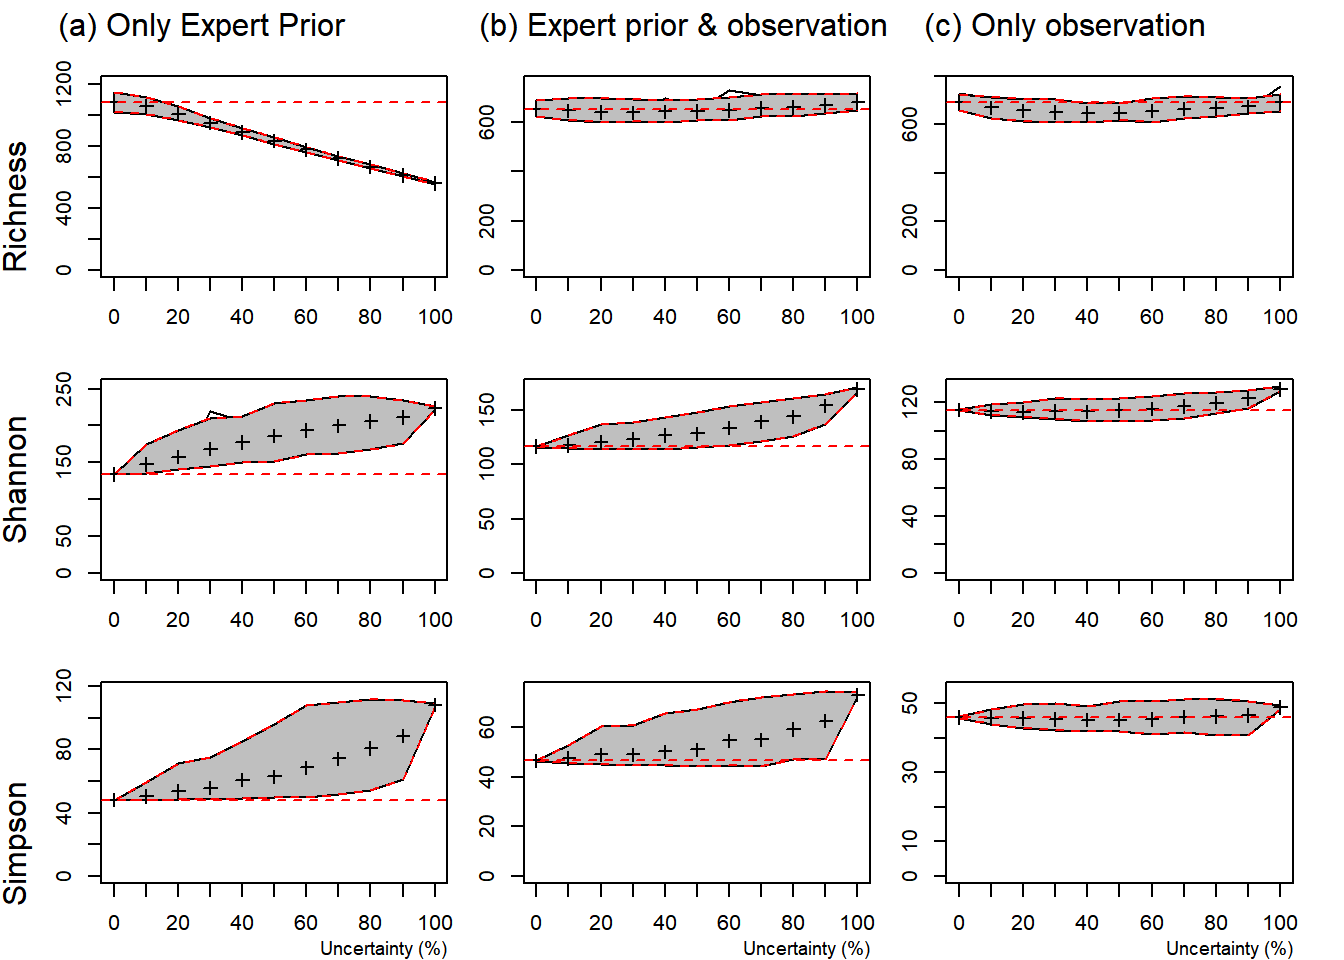
\includegraphics[width=1\linewidth]{TaxonomicUncertainty_files/figure-latex/Fig1-1} \caption{Indices degradation along a taxonomic uncertainty gradient. 95\% envelopes of the Richness, Shannon and Simpson indices calculated through our propagation method along an uncertainty gradient from 0 to 100\% of undetermined species. In (a) Only expert prior is considered to compute the association frequencies, in (b) both expert and observation prior are equally accounted for in the propagation method and in (c) only the observation prior is considered.}\label{fig:Fig1}
\end{figure*}

\begin{quote}
r Fig2, out.width = `60\%', echo=FALSE,fig.cap=``Degradation along a
taxonomic uncertainty gradient of diversity estimated from a reference
field inventories of 2 000 trees. 95\% envelopes of the Richness,
Shannon and Simpson diversities calculated along an uncertainty gradient
from 0 to 100\% of undetermined species.''
\end{quote}

\subsection{Calibrating the sampling
effort}\label{calibrating-the-sampling-effort}

We simulated a gradient of sampling effort for the reference field
inventory, in terms of number of trees required to infer a the vector of
association frequencies \([\phi_v]\), to identify the minimum effort for
reliable diversity estimators. We tested a range of sampling effort from
500 to 22 000 trees randomly selected from the whole inventory (Figure
\ref{fig:Fig3}). The biases of the estimators decreased with the order
of diversity. The richness of reference is not faithfully retrieved
before recovering the whole inventory (Figure \ref{fig:Fig3}\emph{(a)})
but the 95\% confidence interval of the estimator does not exceed 7\% of
the initial diversity. The Shannon and Simpson estimators showed lower
biases, the bias of Shannon estimator falls to 15\% for 2 000 reference
trees (Figure \ref{fig:Fig3}\emph{(b)}) and the bias of Simpson
estimator falls to 6\% (Figure \ref{fig:Fig3}\emph{(c)}).

\begin{figure*}
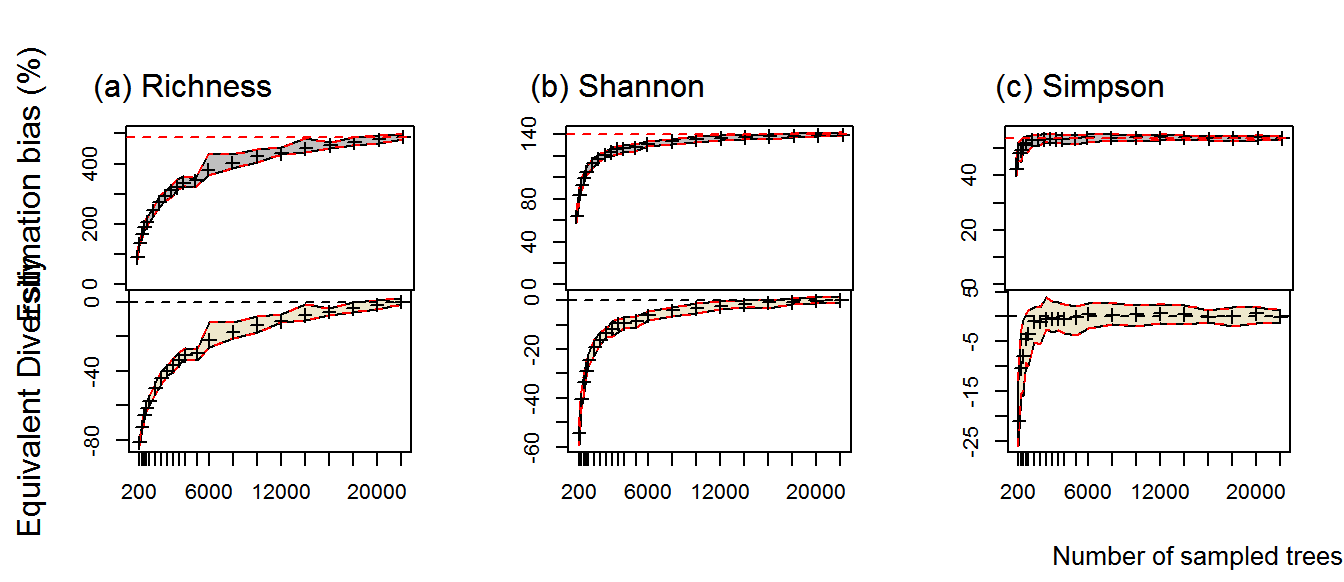
\includegraphics[width=1\linewidth]{TaxonomicUncertainty_files/figure-latex/Fig3-1} \caption{Degradation along a sampling effort gradient of the Richness, Shannon and Simpson diversities estimated for the reference inventory in vernacular names. The propagation method to estimate the diversities is only based on the reference field inventory. Above plots correspond to the estimated diversity in equivalent number of species and below plots correspond to the relative bias of the estimation compared to the value of the reference field inventory. For both dashed lines represent the value of the reference field inventory and crosses and red lines respectively represent the mean, 0.05 and 0.95 quantiles estimated after 1000 iterations.}\label{fig:Fig3}
\end{figure*}

\section{Discussion}\label{discussion}

In this paper we present a method of inventory protocols to correctly
propagate taxonomic uncertainty of vernacular name in the measure of
forest diversity. Our method is based on a Bayesian process which base
is the probability of association between vernacular and botanical
names. The comparison of several methods to build the basic
vernacular-botanical association vectors demonstrated that the biases
and the variability of the diversity estimator were much lower when
reference field inventories are used rather than general
taxa-association table. From this conclusion, we determined the minimum
number of trees for the reference field inventory. To this end we run
the estimation method with a set of association vectors computed from an
increasing number of trees: we found that reference inventories should
be based on a minimum of 2 000 trees, which ensures no more than 10\%
error for Shannon diversity and 1\% error for Simpson diversity. We did
not obtain an unbiased estimator of species Richness but demonstrated a
linear correlation between estimated richness.

\subsection{Prior field inventories for reliable diversity
estimations}\label{prior-field-inventories-for-reliable-diversity-estimations}

We set up a framework providing reliable and accurate diversity
estimations in handling the taxonomic uncertainty of vernacular names
due to their multiple correspondences to botanical species. In the line
of \citet{Guitet2014b} our method propagates the taxonomic uncertainty
to diversity estimators through a Bayesian framework that was either
based on general taxa-correspondence tables or reference field
inventories. We determined the best balance between both dataset in
applying our framework along a gradient of indetermination ratio
\(\big(\cfrac{\text{number of vernacular name}}{\text{number of trees}}\big)\).
Whenever its weight the account of the general taxa-association table
underestimated the Richness and overestimated the Shannon and Simpson
diversities (Figure \ref{fig:Fig1}). The use of general taxa-association
table increases the equitability of the community in inflating the
abundance of rare species at the expense of abundant ones. The
association probabilities computed from this dataset are independent of
species abundance so the vernacular name of a rare species will
indifferently be associated to are or abundant species. The use of a
reference field inventory to the contrary gives vector of association
probability dependent of species abundance and retrieves the real
abundance distribution so the diversity estimator however is much less
biased. A reliable diversity estimator should then be based on reference
field inventory performed beforehand by the working team in the studied
community.

\subsection{Calibration of the reference
inventory}\label{calibration-of-the-reference-inventory}

Reliable diversity estimator should be based on a reference field
inventory ensuring small estimation biases and uncertainty. The
determine the minimum size of this reference inventory we applied our
framework for an gradient of sampling effort, in terms of number of
trees used to compute the association probabilities. We found it
difficult to retrieve the initial richness, as already suggested in
previous analysis comparing random-sampling methods to these based on
restricted inventories \citep{Higgins2004}. However, if the estimator of
richness was biased it varied little and should preserve the ranking of
communities with similar indetermination ratio. This was coherent with
various results linking the whole community richness to that of
communities subsamples \citep{Vellend2008}. The bias of the richness
estimator though is a minor annoyance because for small time and spatial
scale the richness is not necessary the most relevant diversity to
consider \citep{Baraloto2012a, Berry2008a, Cannon1998, Plumptre1996}.
The estimator of Shannon and Simpson diversities were much less biased
and reasonably. Our results showed that from 2 000 trees inventoried
beforehand the Shannon and Simpson estimators respectively had 12\% and
1\% uncertainty.

\section{Conclusion}\label{conclusion}

A keystone for biodiversity conservation is to understand the
determinants of communities assembly, especially in tropical forest
where stands are as complex and species-rich as they are valuable and
uncharted \citep{Magurran1988, Prance1994, Cardinale2012, Sist2015}.
Despite the study of tropical forests structure and composition however
still a need large and intensive sampling in space and time which is
hampered by the important costs of inventories in tropical forests
\citep{Valencia2013}. It is then urgent to develop methods alleviating
the cost of inventories while producing accurate and unbiased estimation
of the diversity. In that respect using vernacular names is promising
because they are easier to attribute, known by the main part of field
workers and proved to bear valuable information. Their reliability at
genus level proved high but variable across tropical regions: it was
estimated around 60-70\% in French Guyana \citep{Hawes2012, Guitet2014b}
and from 32\% to 67\% in Central African \citep{Rejou-Mechain2011}.
Although vernacular names can be used to estimate communities' diversity
they generate significant taxonomic uncertainty due to the multiple
correspondences between botanical and vernacular names. Reliably measure
forest diversity from vernacular names requires setting adapted
protocols and a propagation method of the taxonomic uncertainty. In this
paper we present a method to propagate the taxonomic uncertainty of
vernacular names to the measure of tropical forest diversity. We
calibrated the corresponding inventory protocols to ensure accurate
estimation: at the cost of an initial reference botanical inventory of 2
000 trees Shannon and Simpson diversities are estimated with
respectively 10\% and 1\% accuracy. Our methods is besides workable to
estimate functional and phylogenetic diversities indifferently. The
method is based on reference field inventory and integrates the
specificity of the working team and local forest structure. It is
workable in all contexts and we propose that it be largely applied to
get insights into the issue of vernacular names handling.

%----------------------------------------------------------------------------------------
%	REFERENCE LIST
%----------------------------------------------------------------------------------------

\bibliographystyle{mee}
\makeatletter
% The filename has .bib extension the must be eliminated
\filename@parse{references.bib}
% parse stores the file name in base. Extension starts at the first dot, so don't use dots in file names.
\bibliography{\filename@base}
\makeatother


%----------------------------------------------------------------------------------------

\end{document}
